%------------------------------------------%
% Cannabis Data Science
% Saturday Morning Statistics #30
% Date: 6/25/2022
%------------------------------------------%
\documentclass[xcolor={dvipsnames}]{beamer}

%------------------------------------------%
% Define the title.
%------------------------------------------%
\author{Cannabis Data Science}
\title[\textbf{Saturday Morning Statistics \#30}]{}
\institute[]{\Large Saturday Morning Statistics \#30}
\date{June \nth{25}, 2022}

%------------------------------------------%
% Define the presentation style.
%------------------------------------------%

\hypersetup{pdfpagemode = FullScreen}
\mode<presentation>{
  \usetheme{Boadilla}
  \usecolortheme{orchid}
  \usefonttheme{default}
  \setbeamertemplate{navigation symbols}{}
  \setbeamertemplate{caption}[numbered]
}
\defbeamertemplate*{title page}{customized}[1][]{
  \usebeamerfont{title}\inserttitle\par
  \bigskip
  \vspace{0.5\baselineskip}
  \usebeamerfont{institute}\insertinstitute\par
  \vspace{0.5\baselineskip}
  {\small\usebeamerfont{date}\insertdate\par}
  \usebeamercolor[fg]{titlegraphic}\inserttitlegraphic
}
\setbeamersize{
  text margin left = 0.5in,
  text margin right = 0.5in
}
%------------------------------------------%
% Specify packages.
%------------------------------------------%
\usepackage{amsmath}
\usepackage{caption}
\usepackage[english]{babel}
\usepackage{graphicx}
\usepackage{hhline}
\usepackage[utf8x]{inputenc}
\usepackage{mathtools} % Annotating equations.
\usepackage[super]{nth} % 1st, 2nd, 3rd, etc.
\usepackage{setspace}
\usepackage{subcaption}
\usepackage{tikz}
\usepackage{xparse}

%------------------------------------------%
% Set the theme.
%------------------------------------------%

% Colors
\definecolor{LG}{RGB}{218, 247, 166}
\definecolor{DG}{RGB}{2, 48, 32}

% Palette
\setbeamercolor*{palette primary}{bg=LG, fg=DG}
\setbeamercolor*{palette secondary}{bg=LG, fg=DG}
\setbeamercolor*{palette tertiary}{bg=LG, fg=DG}

%------------------------------------------%
% Define all custom commands.
%------------------------------------------%

% Top space.
\newcommand\T{\rule{0pt}{2.5ex}}

% Bottom space.
\newcommand\B{\rule[-1.25ex]{0pt}{0pt}}

% Blocks.
\newenvironment<>{Block}[2][.9\textwidth]
  {\setlength{\textwidth}{#1}
  \begin{actionenv}#3
    \def\insertblocktitle{#2}\par
    \usebeamertemplate{block begin}}
  {\par\usebeamertemplate{block end}
  \end{actionenv}}

% Balls.
\defbeamertemplate{enumerate item}{largeball}
{\begin{pgfpicture}{-1ex}{-0.65ex}{1.5ex}{1.5ex}
\usebeamercolor[fg]{item projected}
{\pgftransformscale{2.5}\pgftext{\Large\pgfuseshading{bigsphere}}}
{\pgftransformshift{\pgfpoint{0pt}{0.5pt}}
\pgftext{\usebeamerfont*{item projected}\small\insertenumlabel}}
\end{pgfpicture}}

% Fancy arrows.
\NewDocumentCommand\UpArrow{O{2.0ex} O{black}}{%
   \mathrel{\tikz[baseline] \draw [->, line width=0.5pt, #2] (0,0) -- ++(0,#1);}} % Fancy up-arrow.
\NewDocumentCommand\DownArrow{O{2.0ex} O{black}}{%
   \mathrel{\tikz[baseline] \draw [<-, line width=0.5pt, #2] (0,0) -- ++(0,#1);}} % Fancy down-arrow.

% Equations with numbers on the left.
\makeatletter
\newcommand{\LeftEqNo}{\let\veqno\@@leqno}
\makeatother

% No separating line on footnote.
\renewcommand*\footnoterule{}


%------------------------------------------%
% Presentation
%------------------------------------------%
\begin{document}

% Title page.
\begin{frame}{}

% Background.
\tikz[remember picture, overlay]
\node[opacity=1.0, inner sep=0pt] at (current page.center){
  
\includegraphics[height=\paperheight, width=\paperwidth]{images/presentation-cover.pdf}
};

% Title.
\vspace*{3\baselineskip}

\includegraphics[scale=0.375]{images/logo.pdf}
\vspace*{-2\baselineskip}
\titlepage

\end{frame}


%------------------------------------------%
% Introduction
%------------------------------------------%

\begin{frame}{\#30 - MANOVA}

{\bfseries Multivariate analysis of variance (MANOVA)}

\vspace{0.75\baselineskip}
\begin{itemize}

\item Uses the covariance between outcome variables in testing the statistical significance of the mean differences.

\vspace{0.5\baselineskip}

\item Hypothesis: $\sum_{\text{Model}} = \sum_{\text{Residual}}$.

\vspace{0.5\baselineskip}

\item Correlation among dependent variables affects the statistical power.

\end{itemize}

\end{frame}

% Enterage effect?
% Variable interaction


%In the context of NLP, a concordance is a collection of word locations along with their context. You can use concordances to find:
%
%How many times a word appears
%Where each occurrence appears
%What words surround each occurrence


%Collocations are series of words that frequently appear together in a given text.


%------------------------------------------%
% DRAFT MATERIAL
%------------------------------------------%

%\begin{frame}{}
%
%\begin{figure}
%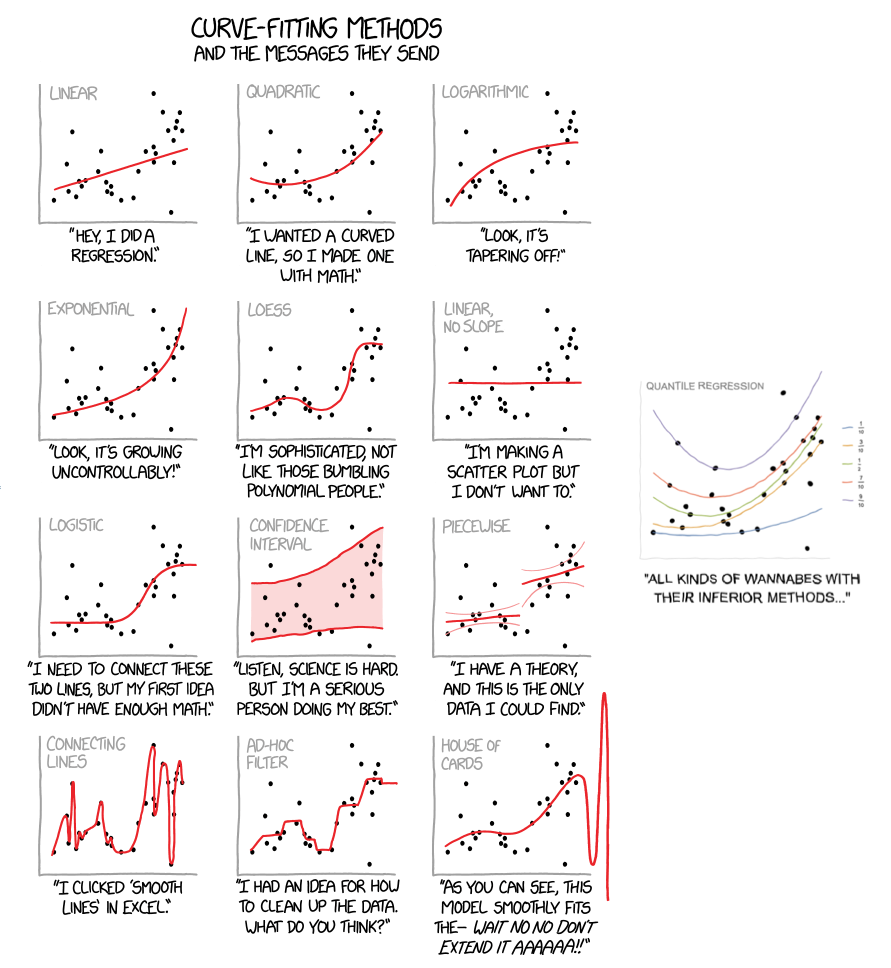
\includegraphics[width=0.725\textwidth]{images/curve-fitting.png}
%\caption*{\tiny\color{Gray} Source: XKCD 2048 as amended by Anton Antonov for a 2019 talk at an R-user meeting in Boston.\\http://www.econ.uiuc.edu/~roger/research/rq/rq.html}
%\end{figure}
%
%
%\end{frame}
%
%
%\begin{frame}{A Brief History in Statistics: Least Absolute Deviation}
%
%{\bfseries Least Absolute Deviation} (LAD) Model
%
%\vspace{0.5\baselineskip}
%\begin{itemize}
%
%\small
%
%\item A special case of quantile regression where q=0.5.
%
%\vspace{0.5\baselineskip}
%
%\item Proposed in 1760 by Roger Joseph Boscovich (1711 - 1787).
%
%\begin{itemize}
%
%\vspace{0.5\baselineskip}
%\item Preceded the least squares method (1805) by fifty years.
%
%\end{itemize}
%
%%\item Developed into the quantile regression by Edgeworth, Roger Koenker, and more.
%
%\end{itemize}
%
%\vspace{1\baselineskip}
%\begin{minipage}{0.45\textwidth}
%\begin{figure}
%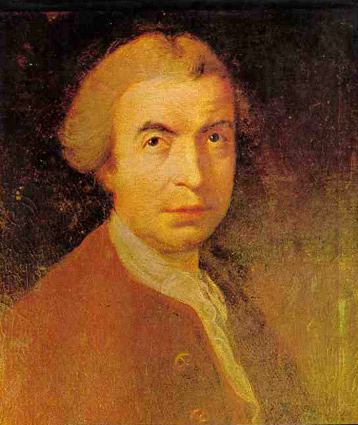
\includegraphics[height=1.25in]{images/bosco.jpg}
%\end{figure}
%\end{minipage}\hspace{0.05\textwidth}%
%\begin{minipage}{0.45\textwidth}
%\begin{figure}
%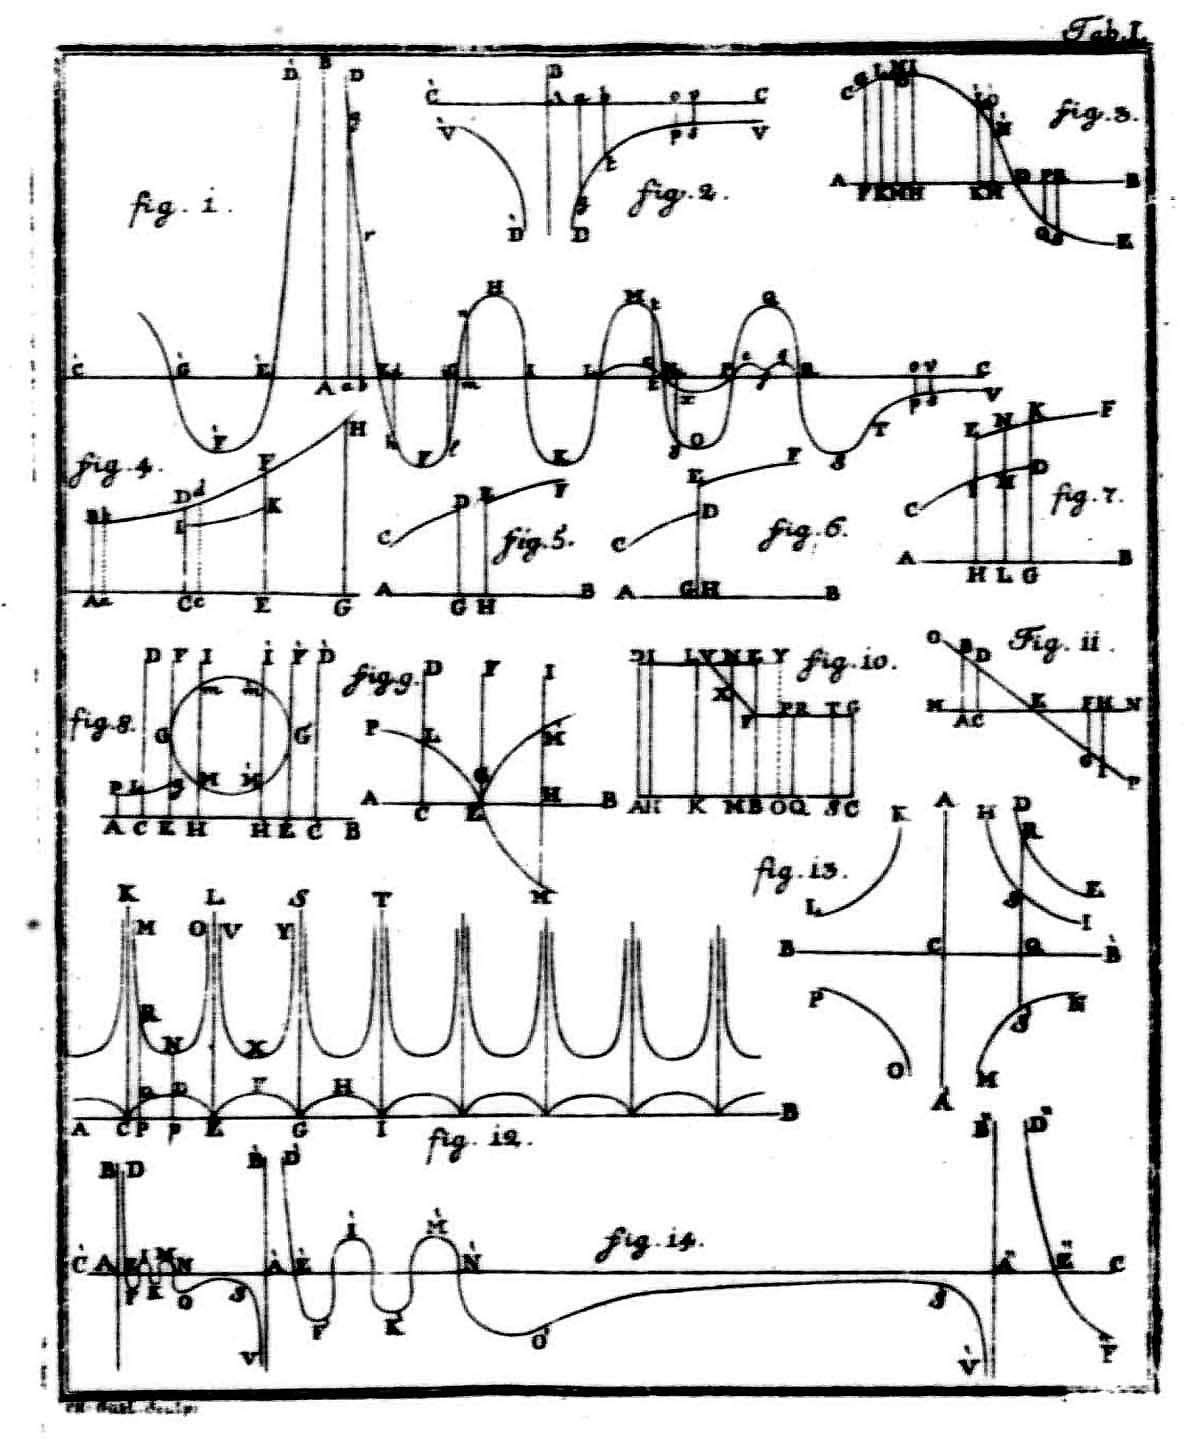
\includegraphics[height=1.25in]{images/bosco-figures.jpg}
%\end{figure}
%\end{minipage}
%
%
%\end{frame}
%
%
%\begin{frame}{Quantile Regression}
%
%A standard regression estimates the mean of the conditional distribution, for example
%
%$$ \hat{y} = \beta_0 + \beta_x \hat{x}. $$
%
%\vspace{1\baselineskip}
%A {\bfseries quantile regression} is a method for estimating conditional quantiles, such as the {\bfseries median}. The conditional $\tau$th quantile is assumed to be a linear function of the explanatory variables:
%
%$$ Q_{Y|X}(\tau) = X\beta_\tau.$$
%
%\end{frame}
% 

%The results obtained from negative sample (left curve) overlap with the results obtained from positive samples (right curve). By moving the result cutoff value (vertical bar), the rate of false positives (FP) can be decreased, at the cost of raising the number of false negatives (FN), or vice versa (TP = True Positives, TPR = True Positive Rate, FPR = False Positive Rate, TN = True Negatives).
% Authors	Sharpr for svg version. original work by kakau in a png
% License: CC BY-SA 3.0
% https://creativecommons.org/licenses/by-sa/3.0



%------------------------------------------%
% Question of the day
%------------------------------------------%

%\section{Hypothesis}
%\begin{frame}{Question and Hypothesis}
%
%% Question of the day
%\begin{center}
%\begin{minipage}{.9\linewidth}
%\begin{Block}{Questions of the day.}
%
%\vspace{.5\baselineskip}
%\begin{itemize}
%
%\item Is the relationship between {\bfseries $\beta$-caryophyllene} and {\bfseries humulene} constant across the conditional distribution?
%
%\vspace{.5\baselineskip}
%
%\item Is the relationship between {\bfseries $\beta$-pinene} and {\bfseries $D$-limonene} constant across the conditional distribution?
%
%\end{itemize}
%
%\vspace{.5\baselineskip}
%
%\end{Block}
%\end{minipage}
%\end{center}
%
%\end{frame}


%------------------------------------------%
% Methodology
%------------------------------------------%


%------------------------------------------%
% Results
%------------------------------------------%



%------------------------------------------%
% Conclusion
%------------------------------------------%


%------------------------------------------%
% Takeaway
%------------------------------------------%
\section{Takeaway}
\begin{frame}{}
\begin{center}

% Thank you.
\begin{minipage}{3.85in}
\begin{center}

\includegraphics[width=.25in]{images/prayer.png} {\Large \textbf{Thank you for coming.}}\\
\end{center}
\vspace*{0.5\baselineskip}

% Insight of the day.
\begin{center}
\begin{minipage}{\linewidth}
\begin{Block}{Insights of the Day}

\vspace{0.5\baselineskip}

\begin{itemize}

\item Statistics is the study of uncertainty.

\vspace{0.5\baselineskip}

\item Statistics and comedy are surprisingly similar.

\vspace{0.5\baselineskip}

\item There may be no more powerful tool than statistics.

\vspace{0.5\baselineskip}

\end{itemize}

\end{Block}
\end{minipage}
\end{center}

\vspace*{1\baselineskip}

\end{minipage}

\begin{center}
Thank you for making Saturday Morning Statistics happen!
\end{center}



\end{center}
\end{frame}
\end{document}
%------------------------------------------%
%------------------------------------------%